%%%%%%%%%%%%%%%%%%%%%%%%%%%%%%%%%%%%%%%%%
% Short Sectioned Assignment
% LaTeX Template
% Version 1.0 (5/5/12)
%
% This template has been downloaded from:
% http://www.LaTeXTemplates.com
%
% Original author:
% Frits Wenneker (http://www.howtotex.com)
%
% License:
% CC BY-NC-SA 3.0 (http://creativecommons.org/licenses/by-nc-sa/3.0/)
%
%%%%%%%%%%%%%%%%%%%%%%%%%%%%%%%%%%%%%%%%%

%----------------------------------------------------------------------------------------
%	PACKAGES AND OTHER DOC%%UMENT CONFIGURATIONS
%----------------------------------------------------------------------------------------

\documentclass[paper=a4, fontsize=11pt]{scrartcl} % A4 paper and 11pt font size

\usepackage[final]{pdfpages}
\usepackage[utf8]{inputenc}
\usepackage[T1]{fontenc} % Use 8-bit encoding that has 256 glyphs
%\usepackage{fourier} % Use the Adobe Utopia font for the document - comment this line to return to the LaTeX default
\usepackage[polish]{babel} % English language/hyphenation
\usepackage{amsmath,amsfonts,amsthm} % Math packages

%\usepackage[usenames,dvipsnames]{color} % Required for custom colors
\usepackage{graphicx}
\usepackage{caption}
\usepackage{subcaption}
\usepackage{listings} % Required for insertion of code
\usepackage{courier} % Required for the courier font

\usepackage[disable]{todonotes}
%\usepackage[disable]{todonotes} % uncomment before final build

\usepackage{algorithm}
\usepackage{algpseudocode}

\usepackage{sectsty} % Allows customizing section commands
\usepackage{url}

\floatname{algorithm}{Algorytm}

\allsectionsfont{ \normalfont\scshape} % Make all sections the default font and small caps

\usepackage{fancyhdr} % Custom headers and footers

\pagestyle{fancyplain} % Makes all pages in the document conform to the custom headers and footers
\fancyhead{} % No page header - if you want one, create it in the same way as the footers below
\fancyfoot[L]{} % Empty left footer
\fancyfoot[C]{} % Empty center footer
\fancyfoot[R]{\thepage} % Page numbering for right footer
\renewcommand{\headrulewidth}{0pt} % Remove header underlines
\renewcommand{\footrulewidth}{0pt} % Remove footer underlines
\setlength{\headheight}{6.6pt} % Customize the height of the header



\numberwithin{equation}{section} % Number equations within sections (i.e. 1.1, 1.2, 2.1, 2.2 instead of 1, 2, 3, 4)
\numberwithin{figure}{section} % Number figures within sections (i.e. 1.1, 1.2, 2.1, 2.2 instead of 1, 2, 3, 4)
\numberwithin{table}{section} % Number tables within sections (i.e. 1.1, 1.2, 2.1, 2.2 instead of 1, 2, 3, 4)

%\setlength\parindent{0pt} % Removes all indentation from paragraphs - comment this line for an assignment with lots of text

%----------------------------------------------------------------------------------------
%	CODE INCLUSION CONFIGURATION
%----------------------------------------------------------------------------------------

\definecolor{MyDarkGreen}{rgb}{0.0,0.4,0.0} % This is the color used for comments
\lstloadlanguages{C++} % Load Cpp syntax for listings, for a list of other languages supported see: ftp://ftp.tex.ac.uk/tex-archive/macros/latex/contrib/listings/listings.pdf
\lstset{language=C++, % UseCpp
        frame=single, % Single frame around code
        basicstyle=\small\ttfamily, % Use small true type font
        keywordstyle=[1]\color{Blue}\bf, % Perl functions bold and blue
        keywordstyle=[2]\color{Purple}, % Perl function arguments purple
        keywordstyle=[3]\color{Blue}\underbar, % Custom functions underlined and blue
        identifierstyle=, % Nothing special about identifiers
        commentstyle=\usefont{T1}{pcr}{m}{sl}\color{MyDarkGreen}\small, % Comments small dark green courier font
        stringstyle=\color{Purple}, % Strings are purple
        showstringspaces=false, % Don't put marks in string spaces
        tabsize=5, % 5 spaces per tab
        %
        % Put standard Perl functions not included in the default language here
        morekeywords={rand},
        %
        % Put Cppl function parameters here
        morekeywords=[2]{on, off, interp},
        %
        % Put user defined functions here
        morekeywords=[3]{test},
       	%
        morecomment=[l][\color{Blue}]{...}, % Line continuation (...) like blue comment
        numbers=left, % Line numbers on left
        firstnumber=1, % Line numbers start with line 1
        numberstyle=\tiny\color{Blue}, % Line numbers are blue and small
        stepnumber=5 % Line numbers go in steps of 5
}

% add new command to include cpp code
\newcommand{\cppscript}[2]{
\begin{itemize}
\item[]\lstinputlisting[caption=#2,label=#1]{#1.cpp}
\end{itemize}

}

%----------------------------------------------------------------------------------------
%	TITLE SECTION
%----------------------------------------------------------------------------------------

\newcommand{\horrule}[1]{\rule{\linewidth}{#1}} % Create horizontal rule command with 1 argument of height

\title{
\vspace*{\fill}
\normalfont
\textsc{Wstęp do algorytmów ewolucyjnych}\\ [20pt]
\horrule{1.5pt} \\[0.4cm] % Thin top horizontal rule
\LARGE Koewolucyjni gracze (Tic-tac-toe)\\ % The assignment title
\horrule{1.5pt} \\[0.1cm] % Thick bottom horizontal rule
\normalsize
\textsc{Specyfikacja Techniczna} \\ [20pt]
\vspace*{\fill}
}

\author{Robert Jakubowski \\Karol Dzitkowski} % Your name

\date{\normalsize\today} % Today's date or a custom date

\begin{document}
\maketitle

\thispagestyle{empty}
\clearpage

\tableofcontents

\clearpage

\section{Opis problemu}
Mierzymy się z problemem napisania sztucznej inteligencji, do gry w kółko i krzyżyk na planszy o wielkości $NxN$ pól.
Podstawą działania sztucznej inteligencji ma być genetyczny algorytm koewolucyjny, różniący się od klasycznego algorytmu ewolucyjnego zależnością oceny osobników od ich interakcji pomiędzy gatunkami. Za pomocą techniki ewolucji program ma nauczyć się grać jak najlepiej. 
\section{Pomysł rozwiązania}
Do implementacji inteligencji w grze użyjemy sieci neuronowej. Poszczególne sieci neuronowe będą osobnikami w populacjach używanych przez algorytm ewolucyjny. Stworzymy dwie osobne populacje osobników dzieląc stworzone wcześniej $K$ sieci neuronowych o losowych wagach na dwie równoliczne grupy - gatunki. Podejście koewolucyjne zastosujemy poprzez przeprowadzanie rozgrywek pomiędzy osobnikami z różnych gatunków. Poprzez funkcję oceny (zależną od wyników rozgrywek), krzyżowanie i mutację będziemy ulepszać sieci neuronowe w obu gatunkach. Najlepszy stopień nauki będziemy próbowali osiągnąć manipulując wielkością populacji, ilością rozgrywanych potyczek oraz prawdopodobieństwami krzyżowania i mutacji. Chcemy wprowadzić również możliwość elitarnego przejścia najlepszych osobników do kolejnej generacji.
\section{Reprezentacja gry}
Planszę reprezentować będziemy jako macierz z polami ponumerowanymi od 1 do $N^2$ od lewej do prawej. \\
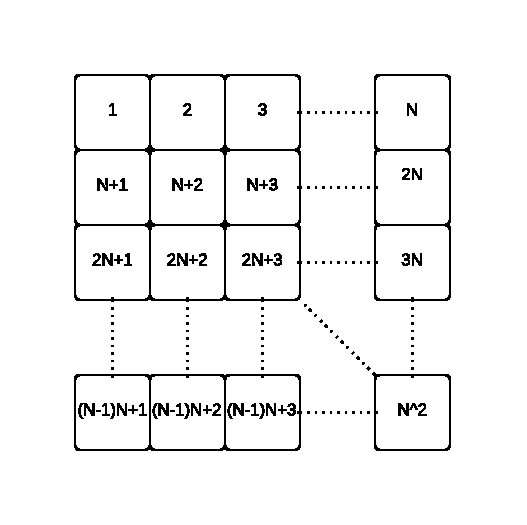
\includegraphics[scale=0.95]{diagrams/CoevolutionaryTicTacToe2} \\
Ułożenie poszczególnych znaków kółka i krzyżyka będziemy reprezentować jako liczby: \\
\begin{itemize}
	\item $0$ -- pole puste
	\item $1$ -- kółko
	\item $2$ -- krzyżyk
\end{itemize}
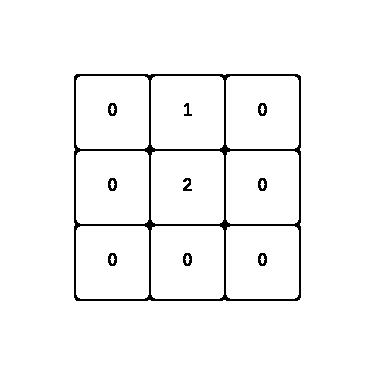
\includegraphics[scale=1]{diagrams/CoevolutionaryTicTacToe3} \\
Potyczki pomiędzy osobnikami będą oceniane w skali punktowej: \\
\begin{itemize}
	\item $1$ -- zwycięstwo
	\item $0$ -- remis
	\item $-2$ -- porażka
\end{itemize}
Chcemy w ten sposób wykreować strategię nieprzegrywającą. \\

\section{Śieć neuronowa}
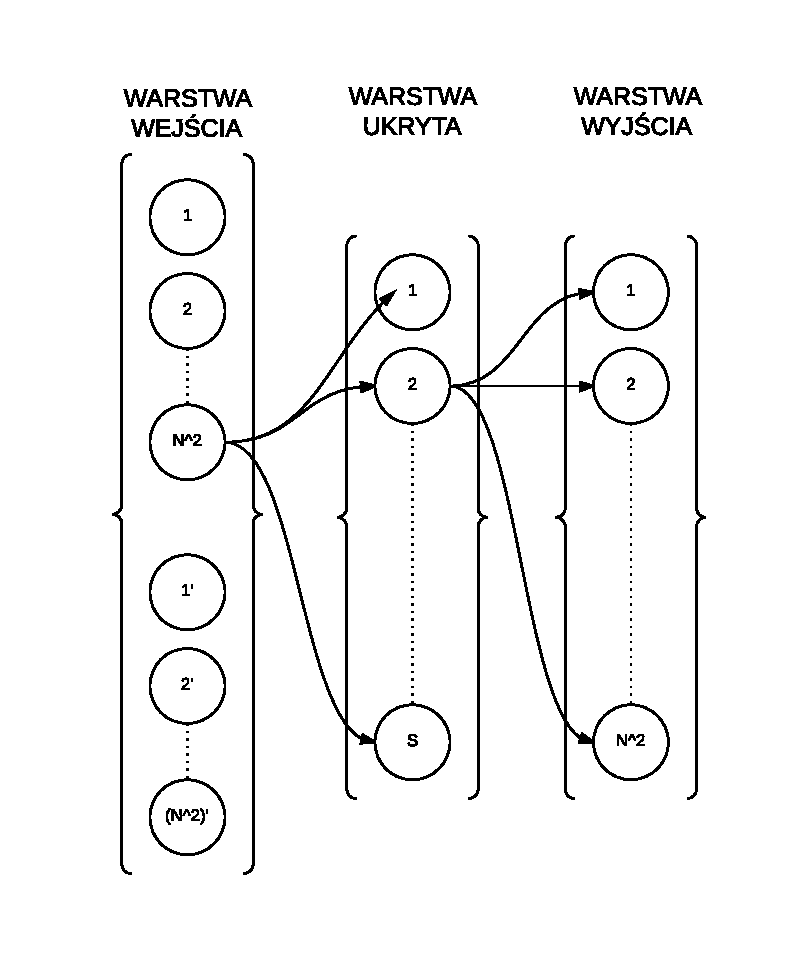
\includegraphics[scale=1]{diagrams/CoevolutionaryTicTacToe} \\
Sieć neuronowa będzie składała się z 3 warstw:
1) warstwy wejścia - zawierającej $2*N^2$ neuronów, gdzie na wejściu każdego będą odpowiednio 0 lub 1 jeśli dane kólko lub krzyżyk jest na danym polu. Zatem mamy $N^2$ neuronów dla krzyżyków i tyle samo dla kółek.
2) Następnie będzie $S$ (wartość ustawiana w konfiguracji) neuronów pośrednich (ukrytych), które będą przetwarzały wejście.
3) W ostatniej warstwie będzie znajdowało się $N^2$ neuronów wyjściowych. Wartość na neuronach wyjściowych będzie wskazywała jak dobre jest ustawienie znaku na danym polu. 
każdy neuron z warstwy 1 będzie miał połączenie z każdym neuronem warstwy 2, natomiast każdy neuron warstwy 2 będzie miał połączenia z wszystkimi neuronami warstwy 3. \\
Algorytm wyeliminuje wszystkie zajęte już pola, a wśród pozostałych wybierze ten dla którego neuron ma największą wartość wyjściową. \\
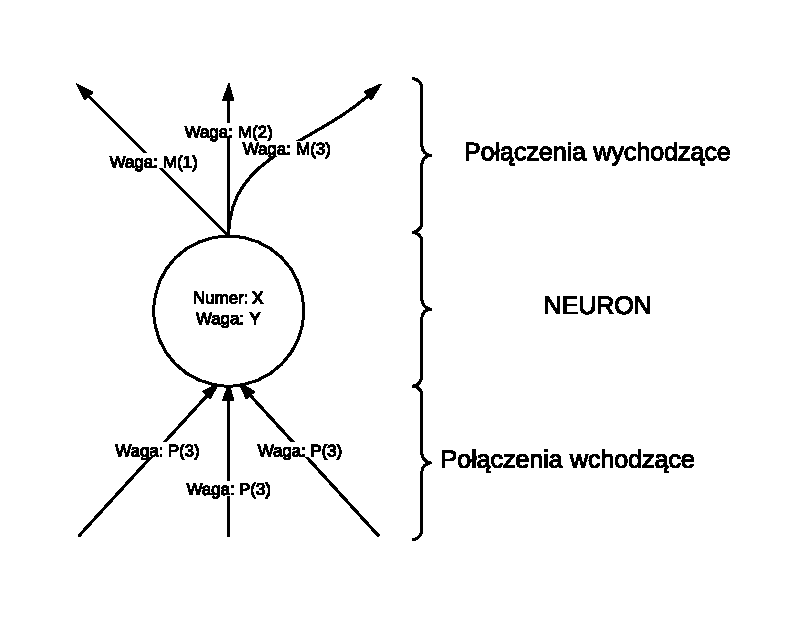
\includegraphics[scale=1]{diagrams/CoevolutionaryTicTacToe4} \\

\section{Generowanie pokoleń}
Kolejne pokolenia będą generowane tak, aby osobniki były coraz lepsze. W naszej aplikacji mają one jak najlepiej radzić sobie w rozgyrwce w kółko i krzyżyk. Należy zapewnić również element losowy, aby rozwiązania nie ograniczyły się tylko do małej części przestrzeni. Zostanie to osiągnięte poprzez zastosowanie krzyżowania oraz mutacji. 

\subsection{Turniej}
W naszej koewolucyjnej metodzie będziemy mieli 2 populacje, które będą ze sobą konkurować, ale nie będą wymieniały się materiałem genetycznym. Osobniki będą rozgrywały partie, ale tylko z osobnikami, które należą do drugiej populacji. Nie będzie możliwy pojedynek dwóch osobników należących do tej samej populacji. Dobre porównanie osobników w danej populacji wymagałoby rozegrania wszystkich możliwych kombinacji spotkań (każdy osobnik z populacji A rozegra po jednym spotkaniu z osobnikami z populacji B). Może się to okazać czasochłonne. Szacujemy, że turniej populacji z 1000 osobników mógłby być czasochłonny. W związku z tym w aplikacji będzie istniało pole, w którym będzie można zdefinowiać ile pojedynków ma rozegrać każdy z osobników. Przeciwnicy będą dobierani losowo. Ilość punktów (suma) zdobytych podczas turnieju będzie określało siłę osobnika.

\subsection{Krzyżowanie}
Proces krzyżowania będzie polegał na stworzeniu osobników. Wszystkie pokolenia będą równoliczne. Do stworzenia nowego osobnika będą potrzebne dwa z poprzedniego pokolenia. Będą one wybierane w losowy sposób, ale rozkład nie będzie jednostajny.

W poprzednim podrzdziale zostało opisane jak będziemy definiować siłę osobników. Wspomnieliśmy już, że nasz algorytm będzie ulepszał populację. W związku z tym podczas losowania osobników do krzyżowania będą faworyzowane osobniki silniejsze. Prawdopodobieństwo wylosowania osobnika ${P_i}$ będzie wyrażało się wzorem:

\begin{equation}
P_i=\frac{p_i + 1}{sum+n}
\end{equation}

gdzie:

\begin{itemize}
	\item ${p_i}$ - liczba punktów zdobyta przez osobnika $i$
	\item $sum$ - suma punktów zdobyta przez wszystkich osobników populacji, do której należy osobnik $i$
	\item $n$ - liczba osobników w populacji
\end{itemize}

Po wyborze osobników, w sposób losowy będą wybierane węzły, które zostaną wybrane z jednego osobnika, a pozostałe zostaną wybrane z drugiego osobnika.

\subsection{Mutacje}
Po etapie krzyżowania nowo utworzone osobniki będą poddane mutacji. Mutacji będzie podlegał jeden węzeł. Nie będzie ona zachodziła zawsze i w programie będzie istniało miejsce do określenia prawdopodobieństwa mutacji. W mutowanym węźle zostanie w sposób losowy zmieniona wartość.

\section{Nauka i testy}
Zaimplementujemy algorytm grający w sposób pseudolosowy i przetestujemy wynik dużej ilości gier nienauczonych osobników populacji (wszystkich po kolei po parę razy). Następnie przeprowadzimy proces nauki i ponownie przeprowadzimy ten sam test. Będziemy badać efekt nauki dla różnych wartości zmiennych w programie takich jak ilość neuronów pośrednich, ilość potyczek czy wielkość populacji aby wybrać optymalne wartości. 


\clearpage

\end{document}